\begin{figure}
	\centering
	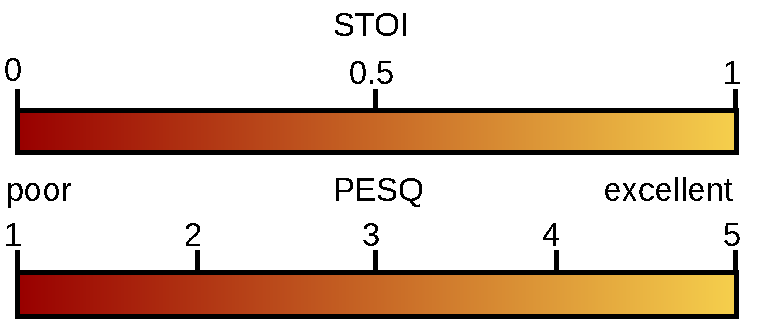
\includegraphics[width=0.5\textwidth]{metrics}
	\caption{\ac{PESQ} and \ac{STOI} metric scales}
	\label{fig:metrics}
\end{figure}

\begin{table}
	\centering
	\caption{mean change STOI and PESQ scores for a subset of the validation set}
	\label{tab:results}
	\resizebox{0.5\textwidth}{!} {
	\begin{tabular}{lrr}
	\toprule
	                      Method &  mean $\Delta $STOI      &  mean $\Delta$PESQ \\
	\midrule
	    Frequency-domain uniform &         0.000793 &        -0.108072 \\
	 Frequency-domain perceptual &        -0.000736 &        -0.222621 \\
	                 Time-domain &         0.001660 &        -0.348682 \\
	\bottomrule
	\end{tabular}

	}
\end{table}

To evaluate the results, two common speech metrics are used: \ac{STOI} and \ac{PESQ}. \ac{STOI} measures speech intelligibility, whereas \ac{PESQ} measures speech quality. Figure \ref{fig:metrics} shows the scaling for each score. Both \ac{PESQ} and \ac{STOI} are intended to be used on segments of speech that are many frames long. In order to measure results in this manner, a long segment of speech is reconstructed using the \ac{WOLA} method \cite{windowSize}. This method was chosen over concatenating adjacent frames because it lessens the severity of discontinuities at frame boundaries. The \ac{WOLA} method consists of reconstructing frames that overlap by a constant number of samples. Reconstructed frames are multiplied by a Hann window. All frames are then added together with respective offsets to create the final reconstructed signal. Table \ref{tab:results} shows the mean change in the speech metric scores for 10 reconstructed random  examples from the validation set. Both the time-domain and uniform weighted frequency-domain networks improve the \ac{STOI} while making the \ac{PESQ} worse. These networks may be useful for tasks such as \ac{ASR} where intelligibility is valued over quality. Notably, the time-domain network achieved both a larger boost in \ac{STOI} and a larger detriment to the \ac{PESQ} than the frequency-domain network. Figure \ref{fig:specs-time} shows spectrograms for the input, target, and the time and uniform frequency models for an example speech sequence. Figure \ref{fig:specs-percep} shows a comparison of input, target, and perceptual/uniform frequency domain models. Unfortunately, it appears that the custom perceptual loss function does not function as desired, reducing both \ac{PESQ} and \ac{STOI} by small margins.

\begin{figure}
	\centering
	\includegraphics[width=0.5\textwidth]{figures/specs-percep.png}
	\caption{Spectrograms of Reconstructed Example (Uniform and Perceptual Frequency Weighting)}
	\label{fig:specs-percep}
\end{figure}

\begin{figure}
	\centering
	\includegraphics[width=0.5\textwidth]{figures/specs-time.png}
	\caption{Spectrograms of Reconstructed Example (Uniform Frequency and Time Domain)}
	\label{fig:specs-time}
\end{figure}
